\graphicspath{{Billeder/}}
\chapter{Test}
\section{Unit tests}
Link til Jenkins - Unit tests: \url{http://ci3.ase.au.dk:8080/job/TeamTyveATMUnitTest/} \newline 

Der er valgt ikke at teste ConsoleLogger.cs, da denne skriver direkte til konsollen, og det er ikke muligt at erstatte statiske metoder. Det vil derfor ikke være muligt at teste om Console.WriteLine() udskriver det korrekte. 

\section{Integrationstests}
Link til Jenkins - Integrationstests: \url{http://ci3.ase.au.dk:8080/job/TeamTyveATMIntegrationTest/} \newline

\textbf{Dependency Tree} \newline
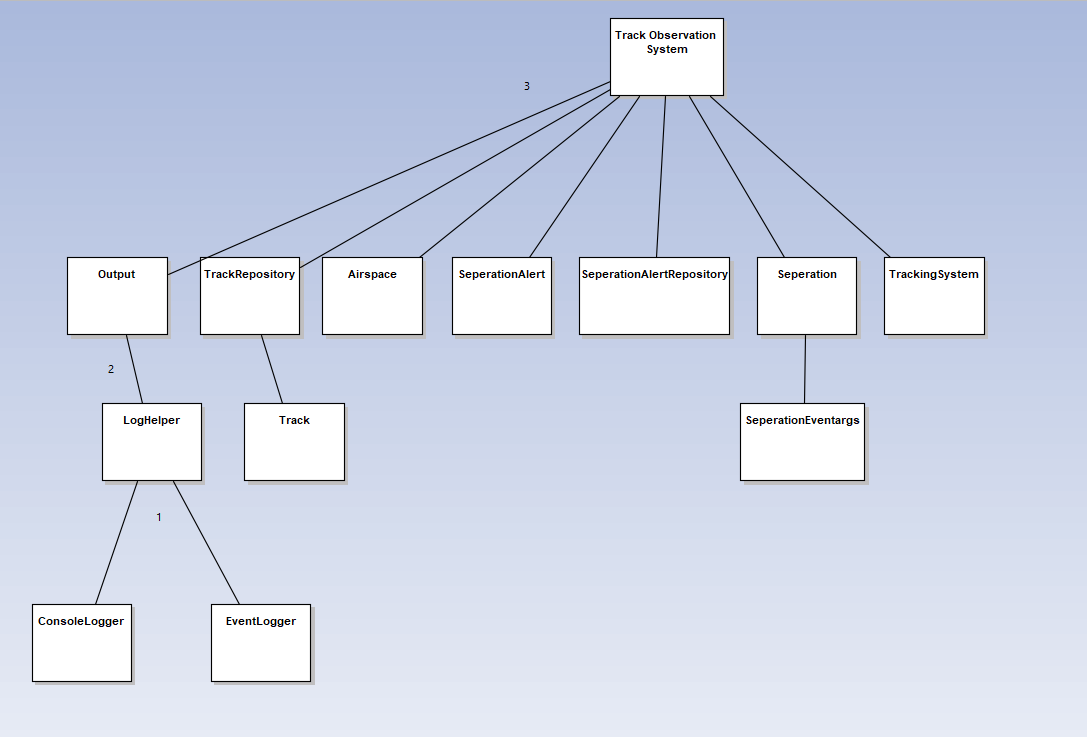
\includegraphics[scale=0.65]{dependencyTree.PNG} \newline
Ovenstående ses dependency-tree for systemet. Der er i alt tre steps, hvor der er valgt at teste det nederste lag først, og derfra bevæge sig op. Altså er bottom up valgt som integrationsstrategi \newline

Denne strategi er valgt grundet at der derved er færre komponenter der skal stubbes, samt at det har virket intuitivt at bruge denne strategi.

Generelt set går bottom up testing ud på at starte fra bunden i det tilhørende dependency tree. De nederste klasser, og derved de klasser der afhænger af mindst vil blive testet først. Hvorfra der hierakisk vil blive testet op igennem træet, indtil alle forbindelser imellem klasserne er blevet tests. Der vil altså blive testet fra submodulerne til hovedmodul(erne).
En af fordelene ved bottom up strategien er at det kan eliminere behovet for anvendelse af stubbe i og med at der ikke er nogle højerestående dependencies at tage højde for. Dog er en af ulemperne ved strategien, at man får testet den overordnet funktionalitet sent i processen, og der derfor er risiko for at man skal lave noget af systemet om, senere end nødvendigt. \newline

\textbf{Integrationsplan} \newline
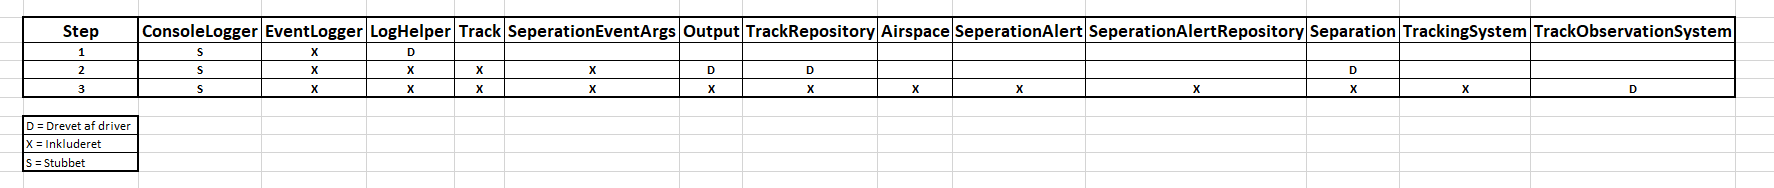
\includegraphics{plan.PNG} \newline
Integrationsplanen viser hvordan de forskellige klasser er inkluderet eller stubbet under de forskellige steps i integrationstesten. Integrationsplanen er lavet med udgangspunkt i dependency træet.

\section{Diskussion}
Til denne hand in var der ikke givet nogle specifikke retningslinjer for hvordan opgaven skulle løses. Dette betød også, at der var stor frihed til hvordan systemet skulle designes. \tabularnewline
Der blev valgt et design, der gjorde at Track Observation System (TOS) - klassen var meget afhængig af de andre klasser, som det også fremgår af det udarbejdede dependency tree. 
Ud fra dette, kan det også ses at det er et ret "horisontalt" system, i og med at TOS indhenter strings og objektifiserer disse. 
Når dette er gjort vil der arbejdes direkte på objekterne igennem de andre klasser, i stedet for at bruge en form for pipes and filters arkitektur, hvor der arbejdes i en vandret orden, og objekterne bearbejdes hen ad vejen i stedet for det hele på én gang. 

Dette blev i starten valgt, grundet at flere ting arbejdede på én gang. Der blev blandt andet tjekket på om flyet var i AirSpace, men også om flyet fløj for tæt på andre fly. \tabularnewline
Set i bakspejlet har det formegentlig været mere testbart at benytte en pipes and filters arkitektur, for at undgå at TOS fik så mange dependencies.

Gruppen fik dog løst det på anden måde og fik et tilfredsstillende resultat.


Der blev benyttet en CI server på Jenkins til at undersøge hvornår et build kunne merges til masteren. \tabularnewline
Dette blev dog ikke benyttet af gruppen, da det meste af systemet blev lavet da medlemmerne sad sammen fysisk på skolen.\tabularnewline
Det ville formegentlig have givet mere værdi i et større team, hvor der arbejdes mere uafhængigt af hinanden. \newline
\pagebreak
\section{Konklusion}
Alt i alt virker systemet som forventet på trods af at de måske ikke har været den optimale løsning der er blevet brugt. \tabularnewline
Set i bakspejlet kunne dette dog være løst ved at have brugt mere tid på design og arkitektur i starten af forløbet.  \tabularnewline
Gruppen har erfaret at det er vigtigt inden at der startes med implementering, at der skal laves en god arkitektur,
som også har fokus på at gøre programmet testbart. \tabularnewline
Gruppen har også erfaret at arkitekturen dermed har stor indvirkning på hvor let det er at lave integrationstest. Med en struktur hvor 
en klasse har for mange afhængigheder, som f.eks. i dette tilfælde med Track Observation System klassen, er det svært at udfører en overskuelig
intergrationstest.
